%% silkpage_coat_of_arms_02.tex — Recursive Arms
%%
%% A more explicitly mathematical SilkPage coat of arms:
%% - Y combinator written as a formal charge
%% - recursive fractal lace built with TikZ recursion
%% - logarithmic spiral / complex-plane allusion for temporal algebra
%% - silk, markup, and lambda carried through the shield
%%
%% compile: xelatex silkpage_coat_of_arms_02.tex

\documentclass[border=24pt]{standalone}
\usepackage{tikz}
\usepackage{fontspec}
\usepackage{xcolor}
\usepackage{amsmath}
\usetikzlibrary{calc}

\newfontfamily\latinfont[
  Path=/System/Library/Fonts/,
  Ligatures=TeX, Kerning=On, Numbers=OldStyle
]{SFNS.ttf}

\definecolor{silkgreen}{HTML}{566E41}
\definecolor{deepgreen}{HTML}{26630A}
\definecolor{sage}{HTML}{DCE5D4}
\definecolor{maroon}{HTML}{57160F}
\definecolor{orange}{HTML}{E97E00}
\definecolor{paper}{HTML}{FFFFFF}
\definecolor{lightgray}{HTML}{DDDDDD}
\definecolor{ink}{HTML}{333333}

\pagecolor{paper}

%% recursive silk branch
\newcommand{\silkbranch}[4]{%
  \ifnum#4>0
    \draw[#1, line width=#2] #3 -- ++(90:#2*16);
    \begin{scope}[shift={#3}]
      \path (90:#2*16) coordinate (tip);
      \draw[#1, line width=#2] (0,0) -- (tip);
      \silkbranch{#1}{#2*0.74}{($(tip)+(132:#2*9)$)}{\numexpr#4-1\relax}
      \silkbranch{#1}{#2*0.74}{($(tip)+(48:#2*9)$)}{\numexpr#4-1\relax}
    \end{scope}
  \fi
}

\begin{document}
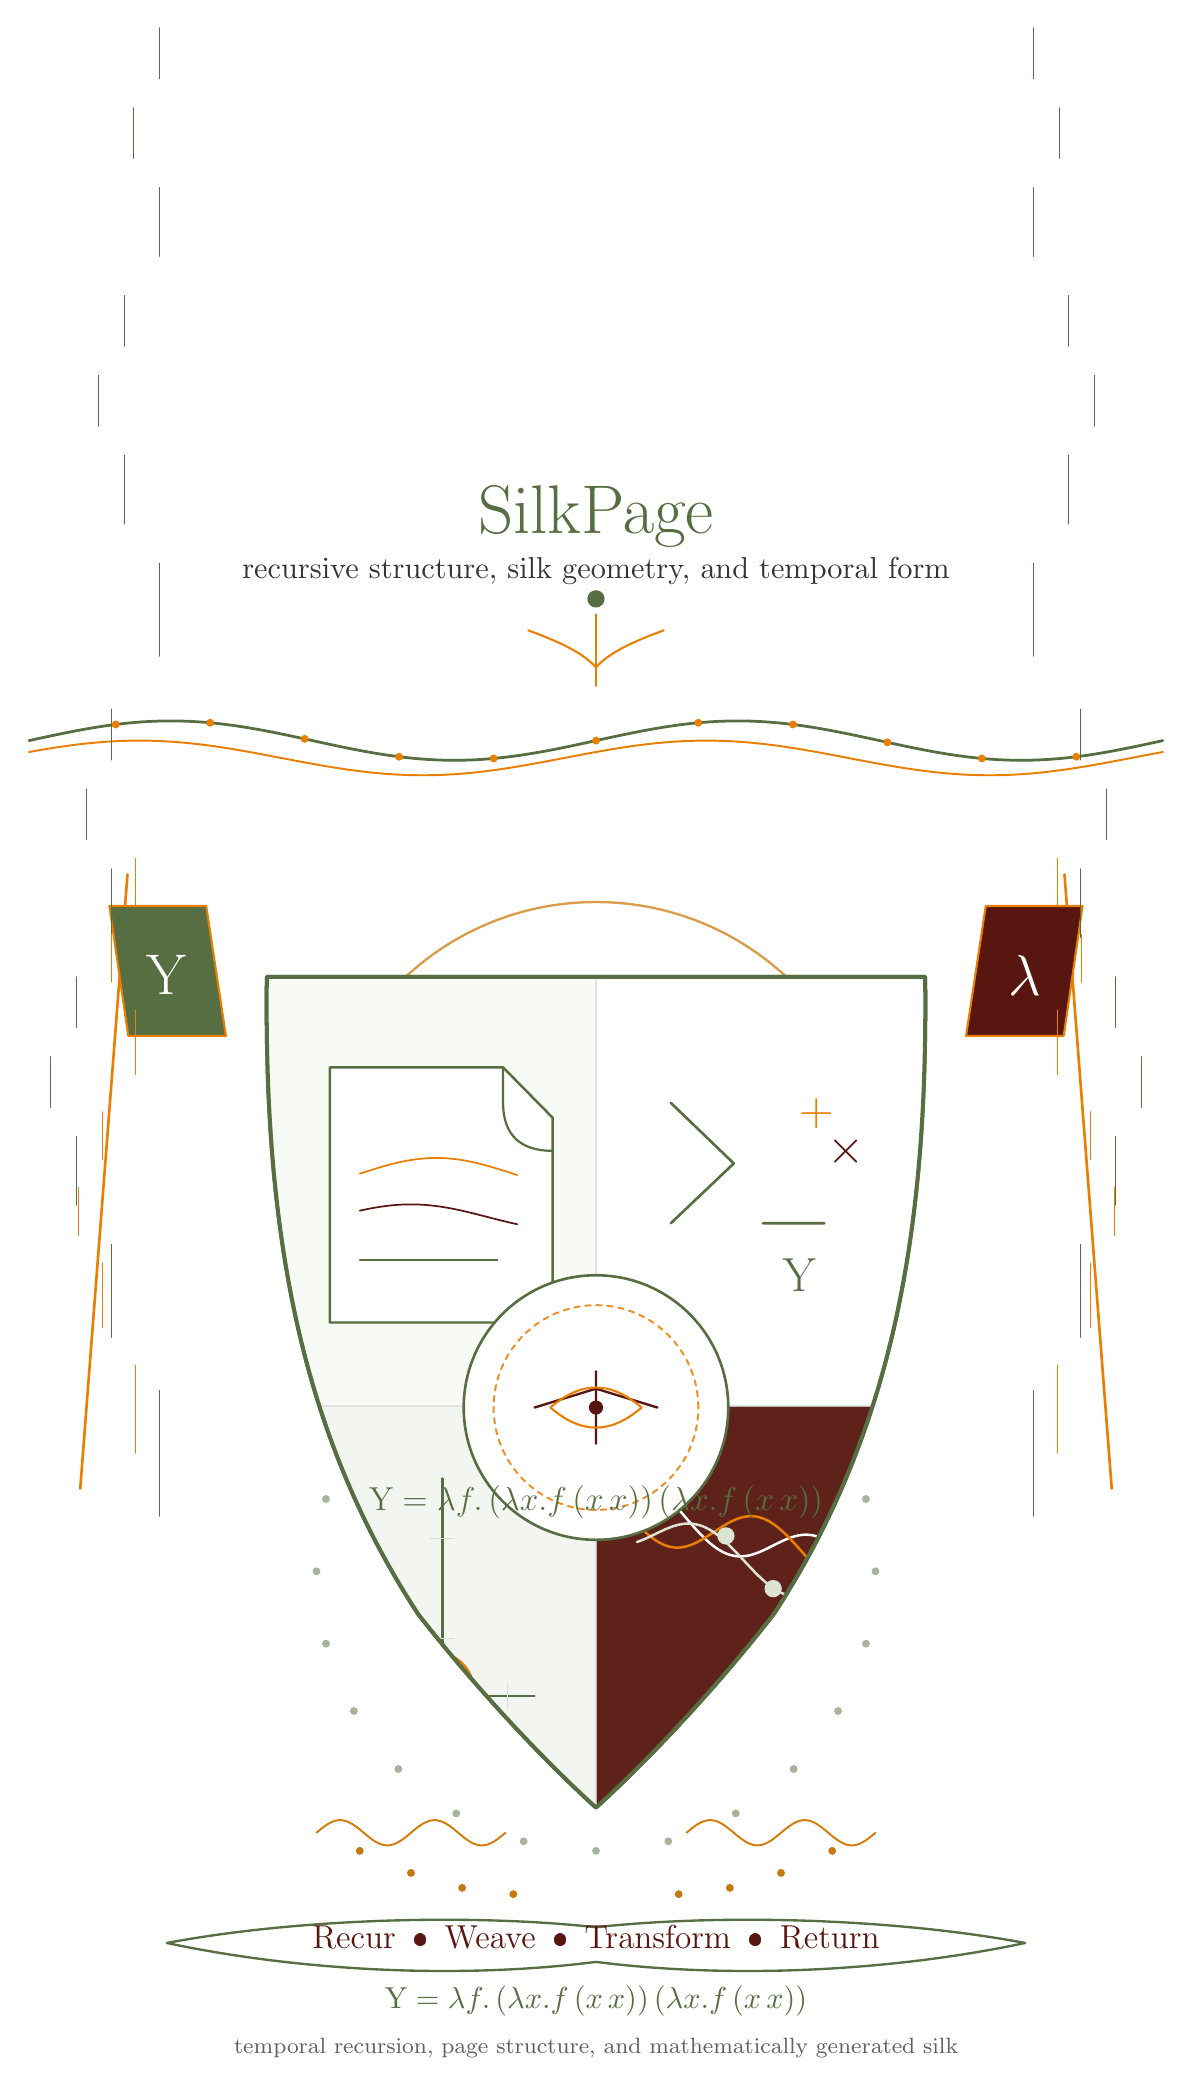
\begin{tikzpicture}[x=1cm,y=1cm,line cap=round,line join=round]

  %% title
  \node[font=\latinfont\fontsize{38pt}{40pt}\selectfont, text=silkgreen] at (0,13.4) {SilkPage};
  \node[font=\latinfont\fontsize{11pt}{13pt}\selectfont, text=ink] at (0,12.7)
    {recursive structure, silk geometry, and temporal form};

  %% crest
  \draw[orange, line width=1.0pt] (0,12.15) -- (0,11.25);
  \fill[silkgreen] (0,12.35) circle (0.11);
  \draw[orange, line width=0.75pt]
    (-0.86,11.95) .. controls (-0.45,11.8) and (-0.16,11.66) .. (0,11.48)
    (0.86,11.95) .. controls (0.45,11.8) and (0.16,11.66) .. (0,11.48);

  %% fractal lace canopy
  \draw[silkgreen, line width=1.0pt, samples=220, smooth, domain=-7.2:7.2]
    plot(\x, {10.55 + 0.25*sin(50*\x)});
  \draw[orange, line width=0.7pt, samples=220, smooth, domain=-7.2:7.2]
    plot(\x, {10.33 + 0.22*sin(50*\x + 20)});
  \foreach \x in {-6.1,-4.9,-3.7,-2.5,-1.3,0,1.3,2.5,3.7,4.9,6.1} {
    \fill[orange] (\x,{10.55 + 0.25*sin(50*\x)}) circle (0.05);
  }

  %% side standards
  \draw[orange, line width=0.95pt] (-5.95,8.85) -- (-6.55,1.05);
  \draw[orange, line width=0.95pt] (5.95,8.85) -- (6.55,1.05);
  \fill[silkgreen] (-6.18,8.45) -- (-4.95,8.45) -- (-4.7,6.8) -- (-5.94,6.8) -- cycle;
  \fill[maroon] (6.18,8.45) -- (4.95,8.45) -- (4.7,6.8) -- (5.94,6.8) -- cycle;
  \draw[orange, line width=0.75pt] (-6.18,8.45) -- (-4.95,8.45) -- (-4.7,6.8) -- (-5.94,6.8) -- cycle;
  \draw[orange, line width=0.75pt] (6.18,8.45) -- (4.95,8.45) -- (4.7,6.8) -- (5.94,6.8) -- cycle;
  \node[font=\latinfont\fontsize{20pt}{20pt}\selectfont, text=paper] at (-5.45,7.58) {Y};
  \node[font=\latinfont\fontsize{21pt}{21pt}\selectfont, text=paper] at (5.45,7.56) {$\lambda$};

  %% recursive side ornaments
  \begin{scope}[shift={(-5.55,0.7)}]
    \silkbranch{silkgreen}{0.10}{(0,0)}{4}
  \end{scope}
  \begin{scope}[shift={(5.55,0.7)}, xscale=-1]
    \silkbranch{silkgreen}{0.10}{(0,0)}{4}
  \end{scope}
  \begin{scope}[shift={(-5.85,1.5)}]
    \silkbranch{orange}{0.07}{(0,0)}{3}
  \end{scope}
  \begin{scope}[shift={(5.85,1.5)}, xscale=-1]
    \silkbranch{orange}{0.07}{(0,0)}{3}
  \end{scope}

  %% orbital ring
  \draw[orange!80!silkgreen, line width=0.85pt, opacity=0.75] (0,4.95) circle (3.55);
  \foreach \a in {0,15,...,345} {
    \fill[sage!60!silkgreen] (\a:3.55) circle (0.05);
  }

  %% shield
  \path[fill=paper, draw=silkgreen, line width=1.45pt]
    (-4.18,7.55)
      .. controls (-4.22,4.2) and (-3.72,1.7) ..
    (-2.26,-0.54)
      .. controls (-1.34,-1.72) and (-0.42,-2.62) ..
    (0,-3.0)
      .. controls (0.42,-2.62) and (1.34,-1.72) ..
    (2.26,-0.54)
      .. controls (3.72,1.7) and (4.22,4.2) ..
    (4.18,7.55) -- cycle;

  \begin{scope}
  \clip
    (-4.18,7.55)
      .. controls (-4.22,4.2) and (-3.72,1.7) ..
    (-2.26,-0.54)
      .. controls (-1.34,-1.72) and (-0.42,-2.62) ..
    (0,-3.0)
      .. controls (0.42,-2.62) and (1.34,-1.72) ..
    (2.26,-0.54)
      .. controls (3.72,1.7) and (4.22,4.2) ..
    (4.18,7.55) -- cycle;

  \fill[sage!20] (-4.3,2.1) rectangle (0,7.7);
  \fill[paper] (0,2.1) rectangle (4.3,7.7);
  \fill[sage!35] (-4.3,-3.2) rectangle (0,2.1);
  \fill[maroon!95] (0,-3.2) rectangle (4.3,2.1);

  \draw[lightgray, line width=0.4pt, opacity=0.8] (-4.18,2.1) -- (4.18,2.1);
  \draw[lightgray, line width=0.4pt, opacity=0.8] (0,7.55) -- (0,-3.0);

  %% upper-left page and silk
  \path[fill=paper, draw=silkgreen, line width=0.9pt]
    (-3.38,6.4) -- (-1.18,6.4) -- (-0.55,5.76) -- (-0.55,3.16)
    -- (-3.38,3.16) -- cycle;
  \draw[silkgreen, line width=0.8pt] (-1.18,6.4) -- (-1.18,5.95)
      .. controls (-1.18,5.55) and (-0.97,5.34) .. (-0.55,5.34);
  \draw[orange, line width=0.62pt, samples=70, smooth, domain=-3.0:-1.0]
    plot(\x, {5.05 + 0.2*sin(185*(\x+3.0)/2.0)});
  \draw[maroon, line width=0.62pt, samples=70, smooth, domain=-3.0:-1.0]
    plot(\x, {4.5 + 0.16*sin(185*(\x+3.0)/2.0 + 30)});
  \draw[silkgreen, line width=0.62pt] (-3.0,3.95) -- (-1.25,3.95);

  %% upper-right derivation signs
  \draw[silkgreen, line width=0.95pt]
    (0.95,5.95) -- (1.75,5.18) -- (0.95,4.42)
    (2.12,4.42) -- (2.9,4.42);
  \node[font=\latinfont\fontsize{16pt}{16pt}\selectfont, text=orange] at (2.8,5.82) {+};
  \node[font=\latinfont\fontsize{16pt}{16pt}\selectfont, text=maroon] at (3.18,5.33) {$\times$};
  \node[font=\latinfont\fontsize{18pt}{18pt}\selectfont, text=silkgreen] at (2.58,3.76) {Y};

  %% lower-left complex plane and spiral
  \draw[silkgreen, line width=0.8pt] (-3.12,-1.58) -- (-0.78,-1.58);
  \draw[silkgreen, line width=0.8pt] (-1.95,-2.56) -- (-1.95,1.18);
  \foreach \x in {-2.78,-2.39,-1.51,-1.12} {
    \draw[lightgray, line width=0.34pt] (\x,-1.74) -- (\x,-1.42);
  }
  \foreach \y in {-2.14,-0.85,0.42} {
    \draw[lightgray, line width=0.34pt] (-2.11,\y) -- (-1.8,\y);
  }
  \draw[orange, line width=1.0pt, samples=220, variable=\t, domain=0:560]
    plot ({-1.95 + 0.09*exp(\t/250)*cos(\t)},
          {-1.58 + 0.09*exp(\t/250)*sin(\t)});
  \fill[maroon] (-1.95,-1.58) circle (0.055);

  %% lower-right woven recursion paths
  \draw[paper, line width=0.9pt, samples=120, smooth, domain=0.52:3.3]
    plot(\x, {0.9 - 0.92*(\x-0.52)/(2.78) + 0.30*sin(160*\x)});
  \draw[orange, line width=0.9pt, samples=120, smooth, domain=0.52:3.3]
    plot(\x, {0.73 - 0.65*(\x-0.52)/(2.78) + 0.32*sin(160*\x + 120)});
  \draw[sage, line width=0.9pt, samples=120, smooth, domain=0.52:3.3]
    plot(\x, {0.54 - 0.82*(\x-0.52)/(2.78) + 0.28*sin(160*\x + 240)});
  \foreach \x/\y in {0.98/0.84,1.65/0.45,2.25/-0.22,2.82/-0.95} {
    \fill[sage] (\x,\y) circle (0.11);
  }

  %% central roundel with Y combinator
  \fill[paper] (0,2.08) circle (1.68);
  \draw[silkgreen, line width=0.95pt] (0,2.08) circle (1.68);
  \draw[orange, line width=0.72pt, opacity=0.85, dash pattern=on 2pt off 2pt] (0,2.08) circle (1.3);
  \draw[maroon, line width=0.85pt]
    (-0.78,2.08) -- (0,2.32) -- (0.78,2.08)
    (0,1.62) -- (0,2.54);
  \draw[orange, line width=0.75pt]
    (-0.58,2.08) .. controls (-0.18,2.42) and (0.18,2.42) .. (0.58,2.08)
    (-0.58,2.08) .. controls (-0.18,1.74) and (0.18,1.74) .. (0.58,2.08);
  \fill[maroon] (0,2.08) circle (0.09);
  \node[font=\latinfont\fontsize{13pt}{14pt}\selectfont, text=silkgreen] at (0,0.88)
    {$\mathrm{Y}=\lambda f.\,(\lambda x.f\,(x\,x))\,(\lambda x.f\,(x\,x))$};

  \end{scope}

  %% redraw shield border
  \path[fill=none, draw=silkgreen, line width=1.45pt]
    (-4.18,7.55)
      .. controls (-4.22,4.2) and (-3.72,1.7) ..
    (-2.26,-0.54)
      .. controls (-1.34,-1.72) and (-0.42,-2.62) ..
    (0,-3.0)
      .. controls (0.42,-2.62) and (1.34,-1.72) ..
    (2.26,-0.54)
      .. controls (3.72,1.7) and (4.22,4.2) ..
    (4.18,7.55) -- cycle;

  %% mathematical lace beneath shield
  \draw[orange!85!silkgreen, line width=0.7pt, samples=120, smooth, domain=-3.55:-1.15]
    plot(\x, {-3.32 + 0.16*sin(360*(\x+3.55)/1.2)});
  \draw[orange!85!silkgreen, line width=0.7pt, samples=120, smooth, domain=1.15:3.55]
    plot(\x, {-3.32 + 0.16*sin(360*(\x-1.15)/1.2)});
  \foreach \x/\y in {-3.0/-3.55,-2.35/-3.83,-1.7/-4.02,-1.05/-4.1,1.05/-4.1,1.7/-4.02,2.35/-3.83,3.0/-3.55} {
    \fill[orange!75!silkgreen] (\x,\y) circle (0.05);
  }

  %% motto and displayed Y combinator
  \path[fill=paper, draw=silkgreen, line width=0.85pt]
    (-5.45,-4.72)
      .. controls (-3.75,-5.08) and (-1.72,-5.18) ..
    (0,-4.96)
      .. controls (1.72,-5.18) and (3.75,-5.08) ..
    (5.45,-4.72)
      .. controls (3.86,-4.42) and (1.66,-4.34) ..
    (0,-4.52)
      .. controls (-1.66,-4.34) and (-3.86,-4.42) ..
    (-5.45,-4.72) -- cycle;
  \node[font=\latinfont\fontsize{11.5pt}{12.5pt}\selectfont, text=maroon] at (0,-4.65)
    {Recur \,•\, Weave \,•\, Transform \,•\, Return};

  \node[font=\latinfont\fontsize{11pt}{13pt}\selectfont, text=silkgreen] at (0,-5.45)
    {$\displaystyle \mathrm{Y}=\lambda f.\,(\lambda x.f\,(x\,x))\,(\lambda x.f\,(x\,x))$};

  \node[font=\latinfont\fontsize{8pt}{9pt}\selectfont, text=ink, opacity=0.78] at (0,-6.05)
    {temporal recursion, page structure, and mathematically generated silk};

\end{tikzpicture}
\end{document}
